\chapter{\ifproject%
\ifenglish Experimentation and Results\else การทดลองและผลลัพธ์\fi
\else%
\ifenglish System Evaluation\else การประเมินระบบ\fi
\fi}

\section{วัตถุประสงค์การทดสอบ (Objective)}
\hspace{2em} การประเมินผลของโครงงานนี้มีจุดประสงค์เพื่อวิเคราะห์ประสิทธิภาพของโมเดล CNN-LSTM \\ ที่พัฒนาขึ้นสำหรับการตรวจจับความผิดปกติ (Anomaly Detection) ใน SWaT dataset โดยมีวัตถุประสงค์สำคัญดังนี้:
\begin{enumerate}
    \item ตรวจสอบความสามารถของโมเดลในการจำแนกสถานะ ปกติ (Normal) และ ผิดปกติ (Anomaly) จากข้อมูล time-series ของ sensor และ actuator
    \item ประเมินประสิทธิภาพตามตัวชี้วัดมาตรฐาน ได้แก่ Precision, Recall, F1-score, Area Under Curve (ROC-AUC, PR-AUC) เพื่อวัดความแม่นยำเชิงสถิติ
    \item วิเคราะห์ Detection Delay และ Latency เพื่อพิจารณาความเหมาะสมในการใช้งานเชิงปฏิบัติการแบบ real-time
    \item เปรียบเทียบผลลัพธ์กับโมเดล baseline เช่น CNN เดี่ยว, LSTM เดี่ยว, Autoencoder เพื่อยืนยันความเหมาะสมของ CNN-LSTM
\end{enumerate}

\section{ข้อกำหนดการทดสอบ (Requirements)}
\subsection{ข้อกำหนดเชิงฟังก์ชัน (Functional Requirements)}
\begin{enumerate}
    \item โมเดลต้องสามารถจำแนกข้อมูล Normal vs Anomaly ได้อย่างถูกต้อง
    \item ระบบต้องสามารถ แจ้งเตือน (Alert System) ได้ทั้งแบบ batch processing และ real-time detection
    \item รองรับการนำเข้าข้อมูลจาก sensor/actuator ที่มีโครงสร้างตาม SWaT dataset
    \item มีการจัดเก็บและนำเสนอผลลัพธ์ในรูปแบบ visualization และ log files (เช่น confusion matrix, error curves)
\end{enumerate}

\subsection{ข้อกำหนดไม่เชิงฟังก์ชัน (Non-Functional Requirements)}
\begin{enumerate}
    \item Accuracy Benchmark: ค่าคะแนน F1-score ≥ 0.9 
    \item ค่า Precision ≥ 0.8 เพื่อจำกัดจำนวนการแจ้งเตือนผิด (False Positive) ให้อยู่ในระดับยอมรับได้
    \item ค่า Recall ≥ 0.9 เพื่อให้มั่นใจว่าโมเดลสามารถตรวจจับเหตุการณ์ผิดปกติได้ครบถ้วน (High Detection Coverage)
    \item Latency: การทำนายผลแต่ละ window ต้องใช้เวลา ≤ 20 ms เพื่อรองรับ real-time operation
    \item Scalability: รองรับจำนวน sensor อย่างน้อย 50 ตัว และ batch size ≥ 64
    \item Usability: ผลลัพธ์ต้องสามารถแสดงในรูป ตารางและกราฟ ที่เข้าใจง่ายต่อผู้ปฏิบัติการ
\end{enumerate}

\subsection{ข้อกำหนดด้านชุดข้อมูล (Dataset Requirements)}
\begin{enumerate}
    \item ใช้ SWaT dataset โดยแบ่งเป็น Normal logs สำหรับการฝึกโมเดล และ Normal + Attack logs สำหรับการทดสอบ
    \item การแบ่งข้อมูลต้องเป็น Training / Validation / Testing sets โดยพิจารณาลำดับเวลาเพื่อป้องกัน data leakage
    \item ต้องทำการ Preprocessing เช่น normalization, sliding window, และการแทนค่าข้อมูลที่หายไป (imputation)
\end{enumerate}

\section{กลยุทธ์การทดสอบ (Testing Strategy)}
\subsection{ประเภทของการทดสอบ (Types of Testing)}
\begin{enumerate}
    \item Functional Testing
    \begin{itemize}
        \item ตรวจสอบความถูกต้องในการจำแนก anomaly ใน test set
    \end{itemize}
    \item Performance Testing
    \begin{itemize}
        \item ประเมินผลด้วย Precision, Recall, F1-score, ROC-AUC และ PR-AUC
        \item วัด latency และ throughput ของระบบ
    \end{itemize}
    \item Comparison Testing
    \begin{itemize}
        \item เปรียบเทียบกับ baseline models ได้แก่ LSTM, CNN
        \item วิเคราะห์ผลลัพธ์เพื่อยืนยันข้อดีของโมเดล CNN-LSTM
    \end{itemize}
\end{enumerate}

\section{ผลการทดสอบเบื้องต้น (Preliminary Results)}

\subsection{ข้อมูลชุดทดลอง}
\hspace{2em} ใช้ข้อมูลจากชุด SWaT A6 ที่ผ่าน preprocessing และ oversampling แล้ว

\begin{enumerate}
    \item ขนาดหน้าต่างเวลา (Window Length): 180 samples ($\approx$ 5 นาที)
    \item ระยะเลื่อนหน้าต่าง (Step): 30 samples ($\approx$ 30 วินาที)
    \item อัตราส่วนคลาสหลัง oversampling: anomaly ≈ 35\%
    \item Split: Train 60\%, Validation 20\% และ Test 20\%
    \item ชุด Validation ใช้ในการเลือก threshold (recall ≥ 0.7)

\end{enumerate}
\newpage
\subsection{ผลการประเมินเบื้องต้น}

\begin{table}[h]
\centering
\begin{tabularx}{\textwidth}{l *{6}{c}}
\hline
Model & \makecell{VAL \\ (PR/ROC)} & \makecell{TEST \\ (PR/ROC)} & \makecell{Accuracy \\ (VAL/TEST)} & Precision & Recall & F1 \\
\hline
CNN-only & 0.609 / 0.643 & 0.434 / 0.686 & 0.563 / 0.724 & 0.50 & 0.42 & 0.46 \\
CNN+LSTM & 0.496 / 0.616 & 0.471 / 0.675 & 0.551 / 0.655 & 0.43 & 0.71 & 0.53 \\
\hline
\end{tabularx}
\caption{ตารางแสดงผลการประเมินเบื้องต้น}
\end{table}

\begin{figure}[h]
\begin{center}
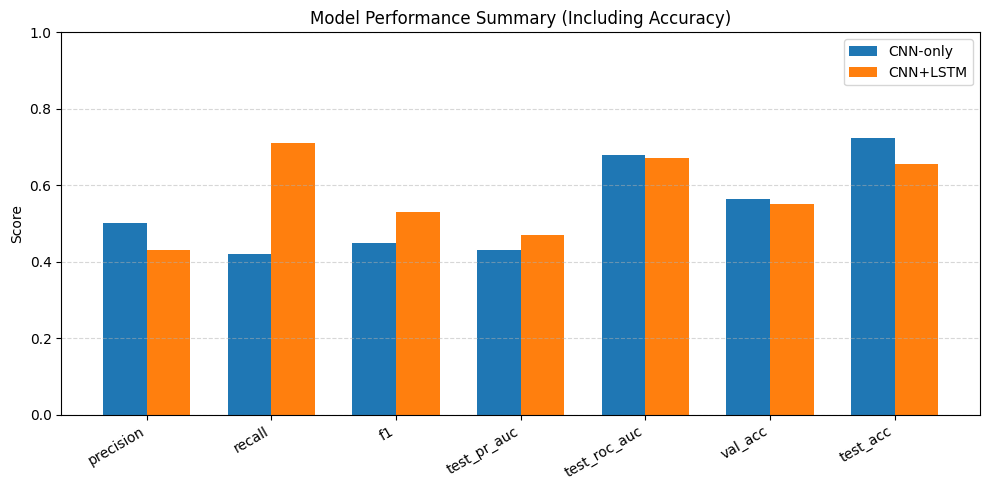
\includegraphics[width=0.8\textwidth]{Image/simple eval.png}
\end{center}
\caption[ผลการประเมินเบื้องต้น]{ผลการประเมินเบื้องต้น}
\end{figure}

Confusion Matrix (Validation / Test):
\begin{enumerate}
    \item CNN-only: [[25,28], [10, 24]], [[53, 10], [14, 10]]
    \item CNN+LSTM: [[22, 31], [8, 26]], [[40, 23], [7, 17]]
\end{enumerate}

\begin{figure}[H]
\begin{center}
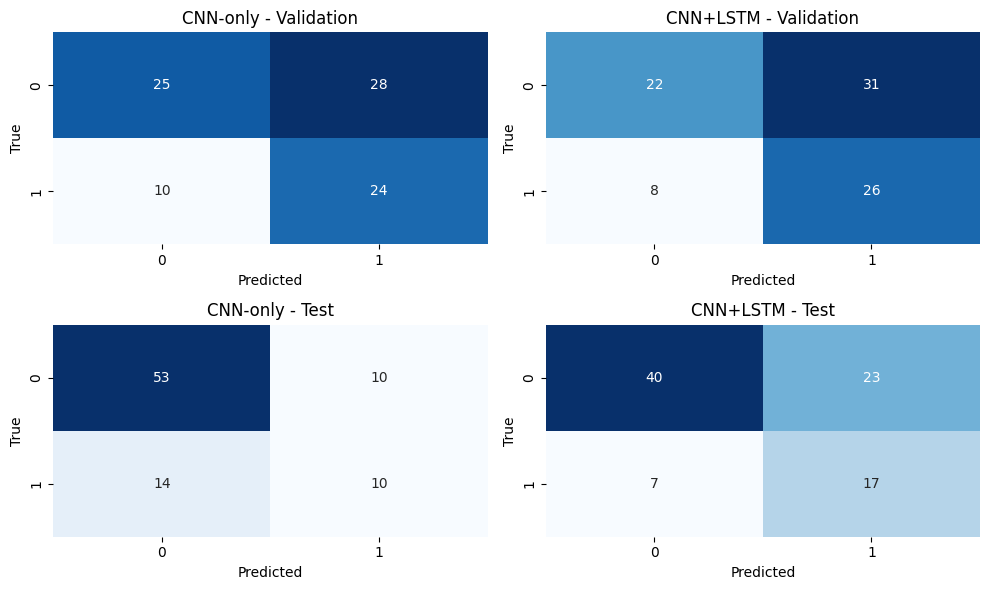
\includegraphics[width=0.8\textwidth]{Image/Confusion Matrix.png}
\end{center}
\caption[Confusion Matrix (Val/Test)]{Confusion Matrix (Val/Test)}
\end{figure}

\newpage
\section{อภิปรายผลการทดสอบเบื้องต้น (Discussion of Preliminary Results)}

\subsubsection{ภาพรวมของผลการทดสอบ}

\begin{enumerate}
    \item โมเดล CNN+LSTM มีค่า Recall สูงกว่า CNN-only อย่างมีนัยสำคัญ (0.708 vs 0.417)
    \item ค่า Accuracy ของ CNN-only อยู่ที่ 0.563 (Validation) และ 0.724 (Test) ในขณะที่ \\ CNN+LSTM มีค่า 0.551 และ 0.655 ตามลำดับ แสดงว่าโมเดลทั้งสองสามารถจำแนกข้อมูลได้ในระดับหนึ่ง แต่ CNN-only มีความแม่นยำโดยรวมสูงกว่า เนื่องจากคาดเดาคลาส “ปกติ” ได้ดี
    \item ค่า ROC-AUC ของทั้งสองโมเดลอยู่ในช่วง 0.67–0.69 แสดงถึงความสามารถในการจำแนกคลาสในระดับน่าพอใจ
\end{enumerate}
อย่างไรก็ตาม โมเดล CNN+LSTM มีแนวโน้มตรวจจับ anomaly ได้ครบถ้วนกว่า แต่เกิดการแจ้งเตือนผิด (False Positive) มากกว่า

\subsubsection{จุดเด่นของโมเดล CNN+LSTM}

\begin{enumerate}
    \item โครงสร้าง BiLSTM ช่วยให้โมเดลสามารถเรียนรู้ลำดับเวลา (Temporal Dependency) ของสัญญาณจาก Sensor ได้ดีกว่า CNN-only
    \item ให้ค่า Recall สูง แสดงถึงความสามารถในการครอบคลุมเหตุการณ์ผิดปกติที่เกิดต่อเนื่องในช่วงเวลา
    \item เหมาะกับการใช้งานในระบบตรวจจับแบบ Real-time ที่ให้ความสำคัญกับ “การไม่พลาดเหตุการณ์ผิดปกติ”
    \item การเพิ่ม LSTM ยังช่วยลดความไวต่อ Noise บางประเภท เนื่องจากสามารถอ้างอิงบริบทของข้อมูลก่อนหน้าได้
\end{enumerate}

\subsubsection{จุดที่ต้องปรับปรุง}

\begin{enumerate}
    \item ค่า Precision ยังต่ำ (~0.4–0.5) แสดงถึงการแจ้งเตือนผิด (false positive) ในระดับสูง
    \item พบแนวโน้ม overfitting จากผลที่ validation ดีกว่า test ส่งผลให้ควรเพิ่ม regularization หรือ dropout
    \item ความไม่สมดุลของข้อมูล (class imbalance) ยังคงเป็นสาเหตุหลักที่ทำให้โมเดล bias ต่อคลาสปกติ
    \item CNN+LSTM มี Accuracy โดยรวมต่ำกว่า CNN-only เนื่องจากทำนาย anomaly มากเกินไป สะท้อนถึงความจำเป็นในการปรับสมดุลระหว่าง Precision และ Recall
\end{enumerate}

\subsubsection{แนวทางปรับปรุงในอนาคต}

\begin{enumerate}
    \item ทดลองใช้ Focal Loss หรือ Class Weighting เพื่อเพิ่มความแม่นยำของการจำแนก anomaly
    \item ปรับ Dropout / L2 Regularization เพื่อควบคุม Overfitting
    \item เพิ่ม Attention Mechanism หรือ Temporal Convolution เพื่อช่วยให้โมเดลเลือกโฟกัส feature สำคัญ
    \item ทดสอบโมเดลบนกระบวนการอื่นใน SWaT (เช่น P1–P6) เพื่อประเมินความสามารถในการ generalize
    \item ปรับ threshold การตัดสินใจให้เหมาะสมกับวัตถุประสงค์เชิงปฏิบัติ เช่น การใช้งาน real-time monitoring
\end{enumerate}